\documentclass[../dissertation.tex]{subfiles}

\begin{document}

\chapter{Monte Carlo Integration, Path Tracing, and Temporal Difference Learning}
\label{chap:technical}

The goal of this section is to a give you as the reader a good understanding of technical concepts which our work relies on. We begin with Monte Carlo integration, as the theory behind how a Monte Carlo approximation can be used to find the true value of an integral forms the mathematical basis of the path tracing algorithm. We then give a full description of the path tracing algorithm and how it relates to the \textit{rendering equation}, as well as pseudo code which we extend upon in chapter \ref{chap:td_deep_sampling}. Finally, we provide a short introduction to Reinforcement Learning and with it, temporal difference learning. This is the foundation of how both NVIDIA and us learn the incident radiance function, but extension of how this applies to path tracing is saved until  chapter \ref{chap:td_deep_sampling}.

\section{Monte Carlo Integration and Importance Sampling}
\label{sec:monte_carlo}
The theory of importance sampling for Monte Carlo integration underpins how noise in images rendered by path tracing can be reduced when using the same number of SPP. Therefore, it is necessary to have a good understanding of Monte Carlo integration and its properties, as well as importance sampling before applying it to path tracing.

\subsection{Monte Carlo Integration}
\label{sec:monte_carlo_approx}
 Monte Carlo Integration is a technique to estimate the value of an integral, equation \ref{eq:integral} represents this integral for a one-dimensional function $f$ between two points $a,b$.

\begin{equation}
\label{eq:integral}
F = \int_a^b f(x) dx
\end{equation}

Monte Carlo integration is used to approximate an integral by uniformly sampling points ($x_i$) to evaluate the integral. These solutions to the integral are essentially averaged to find an approximation to the integral, or in other words, to find the area beneath the curve formed by the function ($f$) within the integral. More formally, basic Monte Carlo integration approximates a solution to an integral using the numerical solution in equation \ref{eq:monte_carlo}. Where $\langle F^N \rangle$ is the approximation of the value of the integral $F$, using $N$ samples and $x_i$ is a sample point \cite{morokoff1995quasi}.

\begin{equation}
\label{eq:monte_carlo}
\langle F^N \rangle = (b - a) \frac{1}{N} \sum^{N-1}_{i=0} f(x_i)
\end{equation}

\begin{equation}
\label{eq:generalized_mc}
\langle F^N \rangle = \frac{1}{N} \sum^{N-1}_{i=0} \frac{f(x_i)}{\frac{1}{(b-a)}} 
 = \frac{1}{N} \sum^{N-1}_{i=0} \frac{f(x_i)}{pdf(x_i)}
\end{equation}

An important property of Monte Carlo Integration is that it produces an unbiased estimate of an integral, meaning the expectation of $\langle F^N \rangle$ is exactly the true value of the integral,$F$ for any $N$ \cite{morokoff1995quasi}. This is presented in equation \ref{eq:unbiased}, where $p_i$ is the probability of a given of a given approximation $\langle F^N \rangle$. Basic Monte Carlo integration only produces a non-bias estimate when sample points $x_i$ are randomly sampled from a uniform distribution. To extend this to \textit{Generalized Monte Carlo} integration, where sample points may be sampled from any distribution, the function evaluated at point $x_i$ must be divided by the Probability Density Function (PDF) over sample points evaluated at $x_i$  ($pdf(x_i)$). Generalized Monte Carlo integration is shown in equation \ref{eq:generalized_mc}, which from here onwards we will refer to as MC integration. Dividing by the PDF ensures the estimate $\langle F^N \rangle$ is unbiased, as areas of the PDF with a high value will be sampled far more, but their contribution weighting ($\frac{1}{pdf(x_i)}$) to final estimate will be lower. Whereas areas of the PDF with a low value will be sampled less, but their contribution weighting to the final estimate will be higher to offset this.

\begin{equation}
\label{eq:unbiased}
\mathbf{E}[\langle F^N \rangle] = \sum_{i = 0}^{k-1} \langle F^N \rangle_i * p_i =  F
\end{equation}

Another important property of MC integration is that by the law of large numbers, as the number of samples ($N$) approaches infinity, the probability of the MC approximation ($\langle F^N \rangle$) being equal to the true value of the integral ($F$) converges to $1$. This law is stated in equation \ref{eq:law_large_numbers}. By this property, MC Integration works well for multidimensional functions, as the convergence rate of the approximation is independent of the number of dimensions. Instead, it is only based on the number of samples used in the approximation ($N$). Whereas this is not the case for deterministic approximation methods, meaning they  suffer from what is known as the curse of dimensionality \cite{bellman1966dynamic}. For path tracing, the integral which is approximated is a 5 dimensional function, hence MC integration is used. This is further described in section \ref{sec:mc_pathtracing}.

\begin{equation}
\label{eq:law_large_numbers}
Pr( \lim_{N \rightarrow \infty} \langle F^N \rangle = F ) = 1
\end{equation}

The standard error of the MC integration approximation decreases according to Equation \ref{eq:mc_error}. Where the standard error describes the statistical accuracy of the MC approximation. Where $\sigma_N^2$ is the variance of the solutions for the samples taken, and is calculated by equation \ref{eq:sample_variance} using the mean of the solutions for the samples taken ($\mu$). Due to equation \ref{eq:mc_error}, it takes four times as many samples to reduce the error of the MC approximation by a half. Also, the square root of the variance is equal to the error of the approximation. Therefore, from here on when we refer to reducing the variance, we also are implying a reduction in the error of the approximation.

\begin{equation}
\label{eq:sample_variance}
\sigma_N^2 = \frac{1}{N-1} \sum_{i=0}^N (f(x_i) - \mu)^2
\end{equation}

\begin{equation}
\label{eq:mc_error}
\text{Standard Error} = \sqrt{Var(\langle F^N \rangle)} = \sqrt{\frac{\sigma_N^2}{N}} = \frac{\sigma_N}{\sqrt{N}}
\end{equation}

\subsection{Importance Sampling for Reducing Approximation Variance}
\label{sec:importance_smapling}

Currently we have only discussed Monte Carlo integration by sampling points $x_i$ to solve the integral using a uniform distribution. However, the purpose of introducing Equation \ref{eq:generalized_mc} was to create a custom $pdf$ which can be used for importance sampling to reduce the variance of the MC approximation. To understand how and why importance sampling works, first observe figure \ref{fig:constant_function} where a constant function is given with a single sample point evaluated for some function $f(x)$. This single sample is enough to find the true value for the area beneath the curve i.e. integrate the function with respect to $x$. This is shown in equation \ref{eq:constant_monte_carlo}, where $p \in \mathbb{R}$ is a constant which can be substituted for $f(x)$.

\begin{align}
\label{eq:constant_monte_carlo}
\langle F^N \rangle & = (b - a) \frac{1}{N} \sum^{N-1}_{i=0} f(x_i)\\
& = (b - a)  \frac{1}{N} \sum^{N-1}_{i=0} p \nonumber \\
& = pb - pa \nonumber
\end{align}

However, figure \ref{fig:non_lin_function} requires many samples to accurately approximate the integral when sampling from a uniform distribution. This is due to the functions complex shape, meaning many samples are required to approximate the area beneath the curve within the MC approximation. Generally, it requires fewer samples to approximate a function which is closer to being constant function \cite{morokoff1995quasi}.

\begin{figure}[h]
\captionsetup{justification=centering}
\centering
\begin{minipage}{.33\textwidth}
    \hspace*{\fill}%
      \begin{tikzpicture}
	    \begin{axis}[
		    axis lines = left,
		    tick style={draw=none},
		    xticklabels={},
		    yticklabels={},
		    xlabel = $x$,
		    ylabel = {$f(x)$},
		]
		%Below the red parabola is defined
		\addplot [
		    color=red,
		]
		{0.1};
		\addplot[mark=*] coordinates {(0,0.1)} node[]{} ;
		
		\end{axis}
	\end{tikzpicture}
     \caption{Constant function\\ with a sample point}
  \label{fig:constant_function}
\end{minipage}
\hspace{8em}
\begin{minipage}{.33\textwidth}
    
  \hspace*{\fill}%

    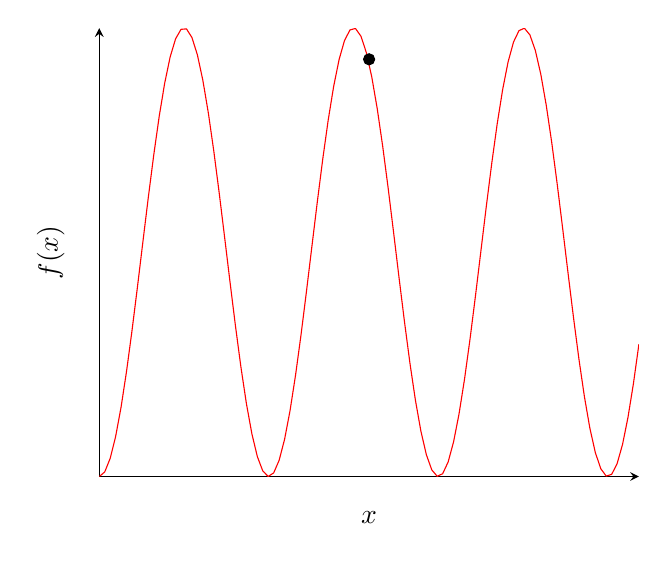
\begin{tikzpicture}
	\begin{axis}[
	    axis lines = left,
	    tick style={draw=none},
	    xticklabels={},
	    yticklabels={},
	    xlabel = $x$,
	    ylabel = {$f(x)$},
	]
	%Below the red parabola is defined
	\addplot [
	    color=red,
	    samples=100,
	]
	{sin(deg(x+5))^2};
    \addplot[mark=*] coordinates {(0,0.93)} node[]{} ;
	\end{axis}
	\end{tikzpicture}  
  \caption{ Non-linear function\\ with a sample point}
  \label{fig:non_lin_function}
\end{minipage}
\end{figure}

Most functions are not constant, however it is possible to turn any function into a constant one. This is exactly what can be done within MC integration. To convert a function $f$ to a constant function, a function $f'$ can be introduced which produces the same output as $f$ for every input, but scaled by a constant $c$ \cite{scratchapixel_2015}. The function $f$ is then divided by $f'$ to produce a constant function, as shown in equation \ref{eq:constant_conversion}.

\begin{equation}
\label{eq:constant_conversion}
\frac{f(x)}{f'(x)} = \frac{1}{c}
\end{equation}

This can be applied to MC integration stated in equation \ref{eq:generalized_mc}, by choosing a PDF  which produces the same output as $f$ for all inputs, but divided by some normalizing constant factor $c$ to ensure the PDF is a probability distribution. Therefore, we are able to calculate the true value of the integral through MC integration as shown in equation \ref{eq:solve_mc_integration}. Where it turns out $\frac{1}{c}$ is true value for the integral in Equation \ref{eq:integral}.

\begin{align}
\label{eq:solve_mc_integration}
\langle F^N \rangle & = \frac{1}{N} \sum^{N-1}_{i=0} \frac{f(x)}{pdf(x)} \\
& = \frac{1}{N} \sum^{N-1}_{i=0} \frac{f(x)}{cf(x)} \nonumber \\
& =  \frac{1}{N} \sum^{N-1}_{i=0} \frac{1}{c} \nonumber \\
& = \frac{1}{c} \nonumber
\end{align}

For most cases, it's not possible to know the correct PDF to sample from which can normalize the function being integrated. However, if one has prior knowledge regarding 'important' regions of the functions input space, it is possible to create a PDF whose shape matches the functions more closely than a uniform PDF. By Important areas of the function input space, we mean areas of the input space which contribute a large amount to the integral of the function.

\begin{figure}[!htb]
\captionsetup{justification=centering}
\centering
\minipage{0.32\textwidth}
\begin{tikzpicture}
	\begin{axis}[every axis plot post/.append style={
	  mark=none,domain=-2:3,samples=50,smooth},
	  axis lines = left,
	  tick style={draw=none},
	  xticklabels={},
	  yticklabels={},
	    % All plots: from -2:2, 50 samples, smooth, no marks
	  axis x line*=bottom, % no box around the plot, only x and y axis
	  axis y line*=left, % the * suppresses the arrow tips
	  enlargelimits=upper,
	  xlabel = $x$,
	  ] % extend the axes a bit to the right and top
	  \addplot [
	  color=red,
	  ]{gauss(0.5,0.8)};
	  \addplot [
	  color=blue,
	  ]{gauss(0.5,1.2)/2};
	\end{axis}
\end{tikzpicture}
  \subcaption{Importance sampling reducing variance}\label{fig:improtance_correct}
\endminipage\hfill
\minipage{0.32\textwidth}
    \begin{tikzpicture}
	\begin{axis}[every axis plot post/.append style={
	  mark=none,domain=-2:3,samples=50,smooth},
	  axis lines = left,
	  tick style={draw=none},
	  xticklabels={},
	  yticklabels={},
	    % All plots: from -2:2, 50 samples, smooth, no marks
	  axis x line*=bottom, % no box around the plot, only x and y axis
	  axis y line*=left, % the * suppresses the arrow tips
	  enlargelimits=upper,
	  xlabel = $x$,
	  ] % extend the axes a bit to the right and top
	  \addplot [
	  color=red,
	  ]{gauss(0.5,0.8)};
	  \addplot [
	  color=blue,
	  ]{0.1};
	\end{axis}
	\end{tikzpicture}  
   \subcaption{Uniform\\ sampling}\label{fig:improtance_uniform}
\endminipage\hfill
\minipage{0.32\textwidth}%
    \begin{tikzpicture}
	\begin{axis}[every axis plot post/.append style={
	  mark=none,domain=-2:3,samples=50,smooth},
	  axis lines = left,
	  tick style={draw=none},
	  xticklabels={},
	  yticklabels={},
	    % All plots: from -2:2, 50 samples, smooth, no marks
	  axis x line*=bottom, % no box around the plot, only x and y axis
	  axis y line*=left, % the * suppresses the arrow tips
	  enlargelimits=upper,
	  xlabel = $x$,
       ] % extend the axes a bit to the right and top
	  \addplot [
	  color=red,
	  ] {gauss(0.5,0.8)};
	  \addplot [
	  color=blue,
	  ]{(-gauss(0.5,1.2) + 0.3)/2};
	\end{axis}
	\end{tikzpicture}  
  \subcaption{Importance sampling increasing variance}\label{fig:improtance_incorrect}
\endminipage
\caption{Graphical representation of a function $f(x)$ (red) and the corresponding PDF $pdf(x)$ (blue) used in the MC integration approximation for the integral of $f(x)$.}
\end{figure}

Figure \ref{fig:improtance_correct} represents a PDF which has a similar shape to the function which is being integrated. Therefore, the variance in the MC integration approximation will be lower then that of the uniform distribution shown in figure \ref{fig:improtance_uniform}. Figure \ref{fig:improtance_incorrect} presents an example where the created probability density function does not resemble the shape of the function which is being integrated. Using this PDF for MC integration would significantly increase the variance in the approximation compared to that from a uniform PDF in figure \ref{fig:improtance_uniform}. This is due to regions which have high importance according to the PDF actually contribute a low amount to the integral of the function $f$, causing the rise in variance of the MC approximation.

\section{Monte Carlo Path Tracing}
\label{sec:mc_pathtracing}
In 1986 James Kajiya introduced the rendering equation and with a it a Monte Carlo integral approximation to the equation \cite{kajiya1986rendering}. This Monte Carlo approximation is essentially what is known as today as Monte Carlo Path Tracing. Here, I will give a detailed explanation of the rendering equation and how Monte Carlo Path Tracing approximates the equation by accurately simulating light transport. As Path tracing is a involves a Monte Carlo integral approximation, importance sampling can be used to reduce the variance in its approximation as described in Section \ref{sec:importance_smapling}.

\subsection{The Rendering Equation}
\label{sec:rendering_equation}

Equation \ref{eq:rendering_equation} is the rendering equation. It calculates the radiance incident from a point $x$ at a given viewing angle $\omega$. Radiance indicates the power of light emitted, transmitted, reflected or received by a surface from a given viewing angle, with units watts per steradian per square metre $(W \cdot sr^{-1} \cdot m^{-2})$. Therefore, by placing a camera in a scene, the radiance incident on the lens from a given surface determines the cameras perceived colour and power of light incident from the surface. These values are used to calculate pixel values in computer image generation. The equation states how to correctly perform  light transport simulation for rendering, and in turn how to accurately simulate global illumination. Therefore, methods which can accurately approximate the rendering equation for any given scene can convert the incident radiance into pixel values to produce realistic rendered images of any given scene. The exact details of how this is done will be described in the next section on the forward path tracing algorithm.

\begin{equation}
\label{eq:rendering_equation}
\underbrace{L_o(x, \omega)}_{\text{Outgoing}} =\underbrace{ L_e(x,\omega)}_{\text{Emitted}} + \underbrace{\int_\Omega L_i(h(x, \omega_i), -\omega_i)  \cdot f_r(\omega_i, x, \omega) \cdot \cos(\theta_i) d\omega_i}_{\text{Reflected}}
\end{equation}
Where:
\begin{conditions}
 L_o(x, \omega)   &  The total outgoing radiance from a 3D point $x$, in the direction $\omega$  \\
 L_e(x,\omega)     &  The emitted radiance from the point $x$\\   
\Omega   &  Hemisphere centred around the normal $n$ of the surface, containing all possible angles $\omega_i$ \\
L_i(y, -\omega_i) & The radiance incident from the intersected position $y$ in direction $\omega_i$\\
h(x, \omega_i)   &  Returns the closest intersected position by firing a ray from $x$ in direction $\omega_i$ \\
f_r(\omega_i, x, \omega)   & The BRDF, describing the proportion of light reflected from $\omega_i$ in direction $\omega$\\
cos(\theta_i)   &  Cosine of the angle between surface normal at point $x$ and the direction $\omega_i$\\
\end{conditions}

The rendering equation is based on the physical law of the conservation of energy, where the outgoing radiance in a given direction ($L_o$) from a point is equal to the emitted light ($L_e$) from the point in the direction, plus the reflected light (the integral) from that point in the direction. The emittance term $L_e$ is simple, it is the light emitted the point $x$ which has been intersected, if this is non-zero a light source has been intersected with. However, the reflected light which is represented by the integral is generally analytically intractable, as it involves summing the contribution of incoming radiance from infinitely many directions in the hemisphere $\Omega$ around the point $x$ ($L_i$). Also, the term $L_i$ is recursive \cite{dutre2004state}, as to calculate the radiance incident in the direction $\omega_i$ from some hit-point say $y = h(x,\omega_i)$, a solution is required for $L_o(y, \omega)$. This concept is represented Figure \ref{fig:recursive_rendering}.

\begin{figure}[h]
\begin{center}
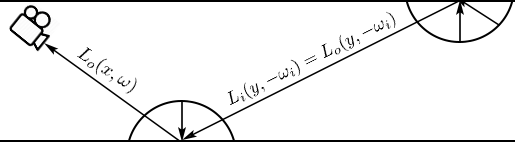
\includegraphics[width=0.7\textwidth]{images/rendering_equation.png}    
\end{center}
\caption{A diagrammatic representation of the recursive nature of the rendering equation. The outgoing radiance ($L_o$) in a given direction $\omega$ from a point $x$ requires an estimation of the incident radiance coming from all angles in the hemisphere around the point, that is $L_i(h(x, \omega_i),-\omega_i) = L_i(y_i, -\omega_i)$ $\forall \omega_i \in \Omega$. To calculate $L_i(y_i, -\omega_i)$ is identical to calculating the outgoing radiance $L_o(y_i, -\omega_i)$ as we assume no radiance is lost along a ray line, hence the $L_o$ is a recursive function. }
\label{fig:recursive_rendering}
\end{figure}

The $f_r$ term in Equation \ref{eq:rendering_equation} is known as the bidirectional reflectance distribution function (BRDF). On a high level, the BRDF describes how a surface interacts with light \cite{glassner2014principles}. Every surface has a BRDF which determines when a ray intersects with that surface at a given incident direction $\omega$, the ratio of reflected radiance in direction $\omega$. Therefore, querying the BRDF for a surface at point $x$ with incident ray direction $\omega'$ and given reflected direction $\omega$, that is $f_r(\omega', x , \omega)$,  a single scalar value is returned. A diffuse and specular surfaces BRDF's are depicted in \ref{fig:brdfs}. A diffuse material reflects light almost equally in all directions for any angle of incidence, an example is paper. Whilst for specular materials, incident rays are reflected in a narrow area around the perfect reflection direction, many metals exhibit specular reflections.

\begin{figure}[h]
\centering
\minipage{0.32\textwidth}
  
\includegraphics[width=\textwidth]{images/diffuse_brdf.png}   
  \subcaption{Diffuse BRDF}\label{fig:diffuse_brdf}
\endminipage\hspace{5em}
\minipage{0.32\textwidth}
  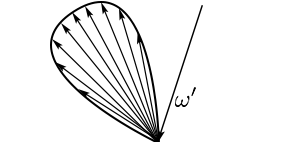
\includegraphics[width=\textwidth]{images/specular_brdf.png}
  \subcaption{Specular BRDF}\label{fig:specular_brdf}
\endminipage
\caption{A representation of both a diffuse surface and specular surface BRDF for a given angle of incidence $\omega'$. The surface point is located where all end of the arrows converge. The arrows indicate a subset of direction possible for the incident ray to be reflected in. All possible directions reflected directions for a ray are defined between the surface point and the line , for an incident direction $\omega'$. The further away a point is on the line, the more likely a ray is to reflected in a direction from the surface point to that point on the line. The diffuse surface is equally likely to reflect a ray in any direction. Whereas, the specular surface favour a small subset are of direction in the hemisphere surrounding the surface point.}
\label{fig:brdfs}
\end{figure}

Another way to think about diffuse and specular materials is do they change in appearance depending on the viewing angle? For example, surface of paper appears to be identical no matter the viewing angle, however a shiny metal ball would appear to reflect what was in front of it which changes depending on the viewing angle, just like a mirror. These differences can be scene in Figure \ref{fig:material_pics}.

\begin{figure}[h]
\centering
\minipage{0.32\textwidth}
  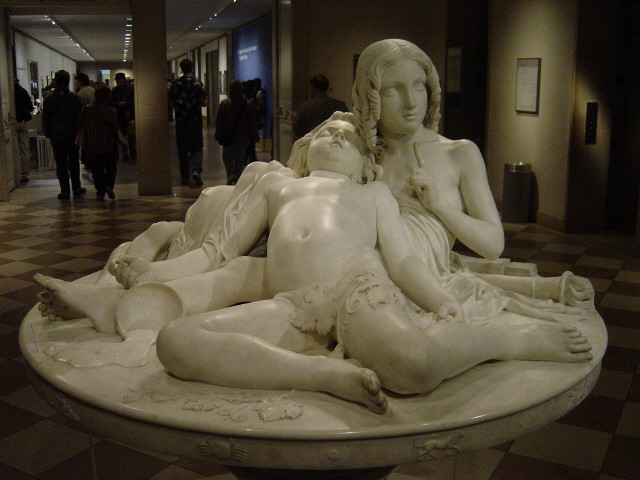
\includegraphics[width=\textwidth]{images/diffuse_sculpture.jpeg}   
  \subcaption{La Table aux Amours, Marble Sculpture}
\endminipage\hspace{5em}
\minipage{0.32\textwidth}
  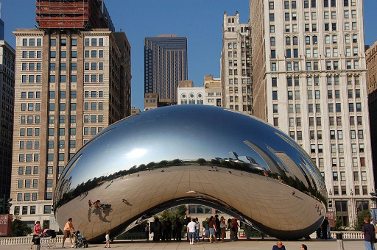
\includegraphics[width=\textwidth]{images/specular_sculpture.jpg}
  \subcaption{Cloud Gate, Stainless Steel Sculpture}
\endminipage
\caption{Two sculptures, one made from a diffuse material (left) and the other from a specular material.}
\label{fig:material_pics}
\end{figure}


A scene comprising of only diffuse materials is generally more computationally expensive to simulate, as one has to simulate rays reflecting in all directions around intersections points with surfaces, compared to a specular scene where only a small subset of directions need to be sampled for each intersection. So, from here on whenever a surface or BRDF is mentioned, assume it is diffuse as my descriptions can be extended to specular materials by restricting ray reflections to a limited set of angles.\\

Finally, as mentioned $cos(\theta_i)$ is the cosine of the angle $\omega_i$ between the normal of the point of the surface intersected with and the angle of incidence. The normal of a surface is the normalized vector that is perpendicular to the surface \cite{normals}. The $cos(\theta_i)$ is a weighting for reflected radiance from a point, where the larger the angle from the normal the smaller the reflected radiance. This simulates how light is spread across the surface, causing less light to be reflected in a direction which is further away from being perpendicular to the surface. The combined BRDF and cosine term in the rendering equation uphold the physical law of conservation of energy, meaning more radiance cannot be reflected from the surface then incident on the surface. This is formally described by Equation \ref{eq:conservation_energy} \cite{glassner2014principles}, where $\omega_r$ represents a direction of reflection.

\begin{equation}
\forall \omega_i, \int_\Omega f_r(\omega_i, x, \omega_r) \cos(\theta_r) d\omega_r \leq 1
\label{eq:conservation_energy}
\end{equation}

\subsection{Path Tracing}

\subsubsection{Monte Carlo Path Tracing}
\label{sec:monte_carlo_path_tracing}

In section \ref{sec:conceptual_path_trace} I already gave a high level overview of the how the path tracing algorithm where many light paths are sampled which consist of shooting a ray from the camera, through a pixel and into the scene to calculate a colour estimate. A pixels colour is then determined by averaging all light paths colour estimates. However I did not detail how to get the colour estimate of a light path. This is exactly what the solution to the rendering equation gives, as $L_o(x,\omega)$ gives the outgoing radiance for each sampled light paths initial direction $\omega$ and intersection point $x$. The radiance is then converted into a pixel colour value. Put another way, $L_o(x,\omega)$ is a pixels colour value where $\omega$ is the direction of the ray when shot from the camera, through the pixel and into the scene. Then $x$ is the position in the scene the ray first intersects with. \\

But how does one solve the rendering equation, as often it cannot be done analytically? This is what Monte Carlo integrating in path tracing is used for. Path tracing solves a slightly different form of the rendering equation to that in \ref{eq:rendering_equation}. To calculate the reflected radiance at point $x$ in the scene for the angle of incidence $\omega$, it is possible to instead calcualte the integral of all light paths which start at the intersection $x$ and reflect round the scene until a light source is intersected with. The proof behind this is detailed in \cite{stanford_graphics}, but conceptually it is simple. Previously the reflected radiance for $(x, \omega)$ was given by the integral of the incident radiance on $x$ with respect to the angle of incidence. To calculate this integral one can trace infinitely rays from the intersection point $x$ in all possible directions $\Omega$ until they high with a light source, the sum of which gives the total amount of incident light on point $x$. Therefore, path tracing solves a variant of the rendering equation to estimate $L_o(x, \omega)$ by integrating over all possible light paths starting from $x$ with respect to the surfaces intersected with. It is this integral which is solved via Monte Carlo integration, the details of which are given in Equation \ref{eq:rendering_eq_monte_carlo}.

\begin{equation}
\label{eq:rendering_eq_monte_carlo}
\begin{array}{l}
    L_o^N(x, \omega) = \frac{1}{N} \sum_{k = 0}^{N-1} L_e(x_0, \omega_0) + (L_i(x_1, -\omega_1) \cdot f_s(\omega_1, x_1, \omega_0) \cdot cos(\theta_{\omega_1})) / \rho_1\\ 
    \\
   \text{Such that}\\
   \\
    L_i(x_i, -\omega_i) = \begin{cases}L_e(x_i, \omega_i) + (L_i(x_{i+1}, -\omega_{i+1}) \cdot f_s(\omega_{i+1}, x_{i+1}, \omega_i) \cdot cos(\theta_{\omega_{i+1}})) / \rho_i & \mbox{if } x_i = \mbox{Light Source}\\ L_e(x_i, \omega_i) & \mbox{otherwise} \end{cases} 
\end{array}
\end{equation} %TODO this is incorrect
Where:
\begin{conditions}
 x_i   & Intersection location of the light path after $i$ reflections in the scene\\
 \omega_i   & Direction of the light path after $i$ reflections in the scene\\
 \rho_i   & Probability density function over reflected ray directions for position $x_i$ and $\omega_i$ angle of incidence
\end{conditions}

In Equation \ref{eq:rendering_eq_monte_carlo} recursive $L_i$ is still present, but the recursion is terminated when the light path intersects with a light source. By the law of large numbers in Equation \ref{eq:law_large_numbers}, the larger the number of sampled light paths ($N$), the closer each pixels approximation will be to the pixels true value as a result of solving the rendering equation. As known from section \ref{sec:rendering_equation}, the rendering equation follows the physical law of energy conservation, and due to this it accurately models light transport simulation for global illumination. Therefore, the more samples used in the Monte Carlo approximation in Equation \ref{eq:rendering_eq_monte_carlo}, the lower the amount of noise in the image \cite{christensen2016path}. An example of this concept applied to a simple forward path tracer is shown in Figure \ref{fig:reduce_noise_spp_example}, and the pseudo code for this forward path tracer to produce a single rendered image is given in Algorithm \ref{alg:forward_path_tracing}.

\begin{figure}[h]
\begin{center}
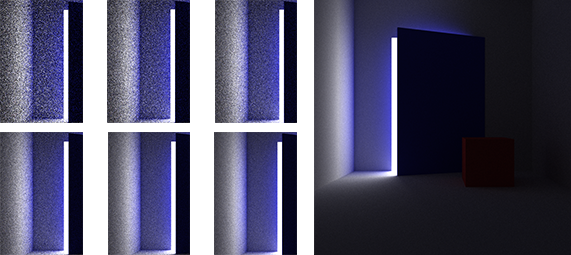
\includegraphics[width=0.99\textwidth]{images/renders/noise_reduction_default/increasing_samples.png}    
\end{center}
\caption{An indirectly illuminated scene from a default path tracer. The grid of image sections represent an increasing number of samples per pixel (SPP), beginning in the top left with 16 SPP, to the bottom right with 512 SPP. The full image on the right is a reference image with 4096 SPP where the Monte Carlo approximation has almost converged for pixel values.}
\label{fig:reduce_noise_spp_example}
\end{figure}

\begin{algorithm}[H]
\label{alg:forward_path_tracing}
\SetKwProg{Fn}{Function}{ }{end}
\SetAlgoLined
 \Fn{renderImage(camera, scene)}{  
   \For{$i = 1$ \KwTo $N$}{
     \For{$p$ \In $camera.screen$}{
         $ray \leftarrow \text{initializeRay}(p, camera)$\\
         \For{$j=1$ \KwTo $\infty$}{
         $(y, \mathbf{n}, L_e) \leftarrow \text{closestIntersection}(ray, scene)$\\
         \If{$\text{noIntersection}(y) \ \Or \ \text{areaLightIntersection}(y)$}{
             $ray.throughput \leftarrow ray.throughput \cdot L_e$\\
             $\text{updatePixelColourEstimate}(p, ray.throughput)$\\
             $\Break$
          }
          $(\omega_i, \rho_i, f_s) \leftarrow \text{sampleRayDirRandomly}(y)$\\
          $ray.throughput \leftarrow ray.throughtput \cdot f_s \cdot (\omega_i \cdot \mathbf{n}) / \rho_i$\\
          $ray \leftarrow (y, \omega_i)$
       }
   }
  }
 }
 \caption{Forward Path Tracer. Given a camera position, scene geometry, this algorithm will render a single image by finding the colour estimate for each pixel using Monte Carlo path tracing. Where $N$ is the pre-specified number of sampled light paths per pixel.}
\end{algorithm}


\subsubsection{Importance Sampling in Path Tracing}

As path tracing is a Monte Carlo method for solving the rendering equation, Importance sampling can be applied in order to reduce the variance pixel colour estimates. In section \ref{sec:importance_smapling} it was shown that by using a probability density function ($pdf$) which closely matches the shape of the function being integrated, the variance in the Monte Carlo estimate is significantly reduced. Applying this to Equation \ref{eq:rendering_eq_monte_carlo}, the term $\rho_i$ which represents the probability density function for sampling the next ray direction at intersection location $x_i$ with angle of incidence $\omega_i$. Currently you can assume that the probability density function $\rho_i$ is uniform. But this can be modified with prior knowledge regarding which directions are more important for continuing a light path in, where an important direction is one which leads to a high contribution of radiance to the pixel estimate.\\

The question now is, can one have any knowledge for which directions contribute the most radiance to the pixels colours value? The answer is yes, and there has been a large amount of research in this which resides in the topic of light transport simulation. The simplest example lies within the rendering equation itself, $cos(\theta_i)$. As previously discussed, this term acts as a weighting for the radiance contribution of outgoing light paths. So, the probability density function $\rho_i$ can also be weighted by $cos(\theta_i)$, which is likely to reduce the pixel value variance. There exists many other methods of retrieving knowledge from the scene to use in importance sampling during rendering. For example, irradiance cahcing \cite{bashford2012significance}, table-driven adaptive importance sampling \cite{cline2008table}, and sequential Monte Carlo adaptation \cite{pegoraro2008towards}. However as discussed in section \ref{sec:motivation}, these previous methods do not effectively reduce the number of zero contribution light paths, meaning their ability to image noise for certain scenes is very limited. Instead, Nvidiai proposed that reinforcement learning can be used for this \cite{dahm2017learning} which is the main inspiration for my work. In the proceeding sections I will discuss in detail how it is possible to apply reinforcement learning for importance sampling in light path construction.

\subsubsection{Existing Methods for Importance Sampling}
% TODO Exisitng methods for importance sampling discussed in more detail

\section{Reinforcement Learning and TD-Learning}
Now that it is clear how Importance sampling light paths can be used to reduce variance in Monte Carlo path tracing, it is time to introduce the concept of reinforcement learning as I will be using this to gain knowledge for this Importance sampling. This section aims to give a quick introduction to reinforcement learning and TD-learning to cover all of the background material of the learning methods I will be using, before describing how they are applied to path tracing in the next section.

\subsection{Markov Decision Processes}
Reinforcement learning is one of the three archetypes of machine learning and it is concerned with finding what action should be taken in a given situation, in order to maximise a numerical reward \cite{sutton2011reinforcement}. This problem is formalized by a finite Markov Decision Process (MDP), which is designed to capture the most important aspects of the problem a learning agent faces when interacting over time with its environment to achieve a goal. A MDP is summarised in \ref{fig:mdp} and can be described in terms of the following:

\begin{itemize}
\item \textbf{Agent} - The learner and decision maker which takes an action $A_t$ in an observed state $S_t$ (where $t$ is the current time step), receiving an immediate numerical reward $R_{t_+1}$ and the next observed state $S_{t+1}$
\item \textbf{Environment} - What the agent interacts with when taking an action $A_t$ in state $S_t$ and produces both $R_{t+1}$ \& $S_{t+1}$ 
\end{itemize}

\begin{figure}[h]
\begin{center}
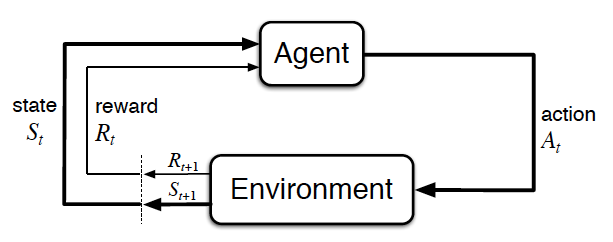
\includegraphics[width=0.5\textwidth]{images/MDP.png}    
\end{center}
\caption{Markov Decision Process \cite{sutton2011reinforcement}}
\label{fig:mdp}
\end{figure}

\noindent
An MDP comprises of the following the following tuple:

$$(\mathcal{S}, \mathcal{A}, p,\gamma)$$
Where:
\begin{conditions}
\mathcal{S}   &  The set of all states\\
\mathcal{A}   &  The set of all actions\\
p   & Probability of receiving reward $r$ and state $s'$ when in the previous state $s$ and action $a$ was taken\\
\gamma   & The discount factor which makes the agent value immediate rewards higher than later ones \\
\end{conditions}

\noindent
An important detail of an MDP which makes it far easier to implement in practice is that any problem modelled by an MDP assumes the Markov property.

\begin{quote}
"The future is independent of the past, given the present." - \textit{Hado van Hasselt, Senior Research Scientist at DeepMind} \cite{introToRL}
\end{quote}

This is expressed mathematically for an MDP in equation \ref{eq:markov_property}. Put simply, the Markov property means the current state captures all relevant information from the history of all previous states the agent has experienced, meaning the history is not needed.

\begin{equation}
\label{eq:markov_property}
p(R_{t+1} = r, S_{t+1} = s' | S_t = s) = p(R_{t+1} = r, S_{t+1} = s' | S_1, .. , S_{t-1}, S_{t})
\end{equation}

\subsection{Goals and Rewards}
The goal thought of for a reinforcement learning agent can change significantly depending on the problem, for example in the case of a game it may be to maximise the total score in one play-through. Or for a robotic space rover it may be to discover the most amount of unseen terrain. However, in terms of an MDP all AI agents goals a described as maximising the total amount of cumulative reward received. This is more formally described by the reward hypothesis \cite{sutton2011reinforcement}

\begin{quote}
Any goal can be formalized as the maximisation of the expected value of the cumulative sum of a received scalar reward signal.
\end{quote}

Once again in the case of an agent learning the best possible action to take for any state in the game (known as the optimal policy), a reward signal could be the points gained by making a certain move. Therefore, to maximise the expected return would be to maximise the number of points received in a play-through.  The return is formally defined in Equation \ref{eq:return} in terms of a reward sequence combined with the discount factor, which as previously mentioned trades off later rewards for more immediate ones. If a discount factor ($\gamma$) is closer to 1 the agent is said to be far sighted, as it gives future rewards a high weighting. Whereas a myopic agent is one which has a discount factor closer closer to 0, as it gives a lower weighting to future rewards for their contribution towards the return $G_t$ \cite{introToRL}. 

\begin{equation}
\label{eq:return}
G_t = R_{t+1} + \gamma R_{t+2} + \gamma^2 R_{t+3} + ... = \sum^\infty_{k=0} \gamma^k R_{t+k+1}
\end{equation}

This formulation works well if the agents interactions with the environment break down easily into sub-sequences \cite{sutton2011reinforcement}, where an agent starts in one of a given set of starting states and takes a series of actions to reach a terminal state. From the terminal state the agent can be reset to one of the starting states to begin learning once again. This applies to path tracing, where the terminal state is one in which the light path has intersected with a light, but this will be discussed in detail in Section \ref{sec:td_light_transport}.

\subsection{Value Function and Optimality}
\label{sec:optimal_value}
All reinforcement learning algorithms I will be considering involve the concept of a value function. There are two kinds of value functions, one which determines the value of being in a given state, the other determines the value of being in a certain state and taking a certain action, known as a state-action pair. The methods I consider are those which use state-action pair value functions, where the value of a state-action pair is defined in terms of the expected return from that state-action pair.

An agent follows a policy $\pi$, which determines how the agent will act in a given state. Formally, a policy is a mapping from states to probabilities of selecting a particular action. When an agent is following policy $\pi$ at time $t$, then $\pi(a|s)$ is the probability that $A_t = a$ if $S_t = s$. Reinforcement learning algorithms state how an agents policy changes from experience. 

The value of a state-action pair $(s,a)$ under a policy $\pi$, is given in Equation \ref{eq:value_function} denoted as $q_\pi(s,a)$,. This value function is commonly known as the action value function for policy $\pi$. Stating 'under policy $\pi$' is important as the value of a given state-action pair depends upon the actions we take onwards from taking action $a$ in state $s$ due to $\pi$. $\mathbf{E}_\pi$ denotes the expected value of a random variable, given that the agent follows policy $\pi$. From this, if one were to keep track of the actual returns received for taking a state-action pair, then as the number of times the state-action pair is chosen tends to infinity, the average of the returns will converge on the true expected value of the return for the state-action pair $q_\pi(s,a)$.

\begin{equation}
\label{eq:value_function}
q_\pi(s, a) = \mathbf{E}_\pi[G_t | S_t = s, A_t = a] = \mathbf{E}_\pi [\sum_{k=0}^{\infty} \gamma^k R_{t+k+1} | S_t = s, A_t = a]
\end{equation}

Now, if you had an AI agent the best way it could perform would be to maximise the expected reward it receives in an episode. In terms of a policies, this is know as the optimal policy which is said to be better then all other policies and agent can follow. Formally, the optimal policy is $\pi$ if $\pi \geq \pi'$ for al possible policies $\pi'$. Where, $\pi \geq \pi'$ if and only if $q_\pi(s,a) \geq q_{\pi'}(s,a)$ for all $s \in \mathcal{S}$ and $a \in \mathcal{A}$. The optimal policy is denoted as $\pi_*$ and the value function following the optimal policy, which is the optimal value function, is denoted $q_*(s,a)$. The optimal value function is defined in Equation \ref{eq:optimal_value}.

\begin{align}
q_*(s,a) & = \max_\pi q_\pi(s,a) \label{eq:optimal_value} \\
 & = \mathbf{E}[R_{t+1} + \gamma \max_{a'} q_* (S_{t+1}, a') | S_t = s, A_t = a]  \label{eq:bellman_optimal}
\end{align}

Equation \ref{eq:bellman_optimal} defines the Bellman optimality equation, which states that the value of a state-action pair under an optimal policy must be equal to the expected return of the immediate reward plus the highest valued state-action pair available from the next state. Intuitively, if the optimal policy is available which is essentially a cheat sheet of what action is most valuable to take in each state. Then the value of a given state-action pair should be equal the immediate reward received by taking the action in the current state, plus the value of the best action to take in the next state given by the cheat sheet/optimal policy. Therefore, if one has the optimal value function, the optimal policy can easily be found by maximising the choice of action $a$ for $q_*(s,a)$  in state $s$ \cite{sutton2011reinforcement}. \\ 

To summarize, the aim from here on is to build an agent which is able to learn the optimal value function, but whilst this is provably possible, it rarely happens in practice. However, the learning methods I will discuss in the next section on TD-learning are able to find a good value function for light path direction sampling.

\subsection{Temporal Difference Learning}
\label{sec:td_learning}

TD-Learning is combination of Monte Carlo and Dynamic Programming reinforcement learning methods for learning the optimal value function from equation \ref{eq:optimal_value}. I will not discuss the details of Monte Carlo and Dynamic Programming methods as they are not investigated as part of my work. However, the reasoning for choosing to study  TD-learning approaches over these two alternative approaches are as follows; TD-learning can perform learning updates of the value function throughout an episode, unlike Monte Carlo approaches which wait until the end \cite{model_free_prediction}. This means TD-learning algorithms can be written in an online learning algorithm \cite{sutton2011reinforcement}. TD-learning can learn directly from experience, as it does not require a true model of the environment in order to learn, unlike Dynamic Programming methods \cite{mdp_dynamic_prog}. This means TD-learning is model-free, avoiding the expense of building the true model of the environment. I will now introduce

I will now introduce three different temporal difference learning methods which are required knowledge for the rest of my work.

\subsubsection*{Sarsa}

Sarsa is a on-policy TD method which learns a good state-action pair valuation function $q_\pi(s,a)$. The Sarsa learning rule is presented in Equation \ref{eq:sarsa}, and I have chosen to present this method first to explain some key concepts TD-learning methods share. Firstly, $Q$ denotes the current value function under policy $\pi$, $q_\pi$. Therefore the left arrow indicates an update in the value of the current estimate $Q$. Also notice, how the current estimate is update upon every time step $t$, this means Sarsa like other TD-learning methods can learn during an episode as previously mentioned. The $\alpha$ term is the current learning rate where $\alpha \in [0,1]$ and $\gamma$ is the discount factor as previously discussed. Finally, Sarsa performs what is known as bootstrapping in the context of reinforcement learning \cite{sutton2011reinforcement}. Bootstrapping is where the  estimate of the valuation function ($Q$), is updated based on some new data by experience, which is the immediate reward $R_{t+1}$. As well as, the current estimate of the valuation function $Q$. Sarsa therefore learns from experience, whereby an action is $A_t$ is taken in state $S_{t}$, leading to an immediate reward $R_{t+1}$ which is used to update the current estimate $Q$.

\begin{equation}
Q(S_t, A_t) \leftarrow Q(S_t, A_t) + \alpha[R_{t+1} + \gamma Q(S_{t+1}, A_{t+1}) - Q(S_t, A_t)]
\label{eq:sarsa}
\end{equation}

The reasoning behind the name Sarsa is that the method uses every element in the quintuple of events, $Q(S_t, A_t, R_{t+1}, S_{t+1}, A_{t_1})$, which makes up a transition between each time step of state-action pairs. Sarsa is an on-policy TD-learning method, as to choose the next action to take in the next state ($Q(S_{t+1}, A_{t+1}$) the policy is used. Sarsa is proven to converge on the optimal value function $q_*$ when the policy $\pi$ remains constant. \\

To make Sarsa learning and TD-learning in general more concrete, imagine a robot with a camera whose goal it is to manoeuvre to the end of a corridor. Each time step is the point when a new frame is rendered on the camera, and the state is the image displayed by the camera. The robots actions consist of moving a short distance in a set of four different direction. If the robot were to learn using Sarsa, the robot would have a large table storing the value of each state-action pair $Q(S_t, A_t)$, which represents the current value function. The robot would then select an action at each time step according to the policy $\pi$ to receive a reward signal based on its distance to the end of the corridor. The robot would then perform a lookup on the large table indexing with the action it took in the state it was in and perform the update rule in \ref{eq:sarsa}. This large table representing the current estimate of the optimal value function is also know as a Q-table, where each value in the table is known as a Q-value, $Q(S_t, A_t)$. By following a suitable policy, the robot will over time will keep updating its Q-values to improve
its estimate of $q_\pi(s,a)$.

\subsubsection{Q-Learning}

Q-learning is very similar to Sarsa except it is an off-policy TD-learning algorithm. Also, if all state-action pairs are visited infinitely many times, it is proven that Q-learning can converge on the optimal policy $q_\pi(s,a)$ faster then Sarsa, therefore it is generally a preferred method. The learning rule is displayed in Equation \ref{eq:q_learning}, where rather then following a policy $\pi$ to select the action to update with, the maximum value of the highest valued action in the next state is selected ($\max_a Q(S_{t+1}, a$). This means the agent following policy $\pi$ will still choose its actions in a state based on $\pi$, however when it update its valuation function $Q$, the action chosen to update with may not necessarily be the same as the action chosen. Hence, Q-learning is an off-policy TD-learning algorithm.

\begin{equation}
Q(S_t, A_t) \leftarrow Q(S_t, A_t) + \alpha[R_{t+1} + \gamma \max_aQ(S_{t+1}, a) - Q(S_t, A_t)]
\end{equation}

\subsubsection{Expected Sarsa}

Expected Sarsa is a TD-learning algorithm which is generally found to be superior to both Q-learning and Sarsa in practice \cite{sutton2011reinforcement}. It is very similar to Q-learning, but instead of using the maximum value of the next state-action pairs it takes the expected value over them. This means Expected Sarsa takes into account how likely each action is under the current policy as shown in Equation \ref{eq:expected_sarsa}. Where $\pi(a | S_{t+1})$ returns the probability of selecting action $a$ in state $S_{t+1}$, while following the policy $\pi$. Note, Expected Sarsa may be used as either an on-policy of off-policy algorithm, for example if the policy $\pi$ was set to the greedy-policy used in Q-learning, the learning rule would become identical to that of Q-learning. Therefore, Expected Sarsa generalizes over Q-learning. Expected Sarsa also reduces the variance in the value function approximation compared to that of Sarsa, as the expectation taken over the current valuation estimate for state-action pairs used.

\begin{align}
Q(S_t, A_t) &  \leftarrow Q(S_t, A_t) + \alpha [R_{t+1} + \gamma \mathbf{E}[Q(S_{t+1}, A_{t+1}) | S_{t+1}] - Q(S_t, A_t)]\\
 & \leftarrow Q(S_t, A_t) + \alpha [R_{t+1} + \gamma \sum_a \pi(a| S_{t+1}) Q(S_{t+1}, a) - Q(S_t, A_t)]
 \label{eq:expected_sarsa}
\end{align}

\subsection{Exploration vs Exploitation}
\label{sec:exploration_vs_exploitation}

Up to now I have formally introduced what reinforcement learning is, including what the optimal value function is and different ways to learn it. As for the TD-learning methods presented so far, I have not discussed any details about the kind of policy an agent should use to select actions in the process of learning. Deciding on this policy is very influential on our agents performance, as the agent needs to gather enough information about its environment to make the best overall decisions. Therefore, online decision-making requires a fundamental choice to be made by the agent every time it chooses to take an action \cite{exploration_vs_exploitation}. This is between the following:

\begin{itemize}
\item \textbf{Exploration}: Maximise the agents performance based on the current knowledge available
\item \textbf{Exploration}: Gain more knowledge about the environment
\end{itemize}

This means a good learning strategy for an agent may be to sacrifice short-term performance to maximise it in the long-term. This applies directly to the policy used in TD-learning methods. Initially exploration is the most important to quickly gain a broad amount of knowledge about the environment and opening up more specific areas for further exploration. Then over time the policy should favour exploitation more and more by taking known higher valued actions. An example of this kind of policy is the decaying $\epsilon$-greedy policy \cite{sutton2011reinforcement}. This policy maintains the current value of $\epsilon \in [0,1]$ and involves sampling a random number $x \in [0,1]$, then if $x > \epsilon$ exploitation occurs, else exploration. By exploitation it is common practice to choose the current highest valued action, whereas exploration involves choosing one at random. Overtime $\epsilon$ is decreased to match the behaviour of increasing exploitation as more knowledge is gained.

\section{Linking TD-Learning and Light Transport Simulation}
\label{sec:td_light_transport}
I will now to link together the concepts introduced so far in this chapter to derive a way of finding the outgoing radiance from position $x$ in direction $\omega$ ($Q(x, \omega)$), based on the TD-learning method Expected Sarsa. I incorperate this learning rule later into Nvidia's online reinforcement learning path tracing algorithm, which uses the learned $Q(x, \omega)$ values for importance sampling directions in light path construction \cite{dahm2017learning}.\\

First, the Expected Sarsa learning rule's summation over the set of all actions $\mathcal{A}$ can be represented as an integral with respect to an action $a$, as shown in Equation \ref{eq:sarsa_integral}. This implies the action space is continuous:

\begin{align}
Q(S_t, A_t) & \leftarrow Q(S_t, A_t) + \alpha [R_{t+1} + \gamma \sum_a \pi(a| S_{t+1}) Q(S_{t+1}, a) - Q(S_t, A_t)]\\
& =  (1 - \alpha) \cdot Q(S_{t},A_t) + \alpha \cdot \left( R_{t+1} + \gamma \sum_a \pi(a|S_{t+1}) Q(S_{t+1}, a) \right)\\
& = (1 - \alpha) \cdot Q(S_{t},A_t) + \alpha \cdot \left( R_{t+1} + \gamma \int_\mathcal{A} \pi(a|S_{t+1}) Q(S_{t+1}, a) da \right)
 \label{eq:sarsa_integral}
\end{align}

Recall the rendering equation from section \ref{sec:rendering_equation} describes the radiance in an outgoing direction $\omega$ from point $x$ is equivalent to the emitted radiance in the direction plus the reflected radiance in the direction. 

\begin{equation}
L_o(x, \omega) = L_e(x,\omega)  + \int_\Omega L_i(h(x, \omega_i), -\omega_i)  \cdot f_r(\omega_i, x, \omega) \cdot \cos(\theta_i) d\omega_i \nonumber
\end{equation}

\noindent
Now, by matching  terms from the rendering equation to the Expected Sarsa learning rule in Equation \ref{eq:sarsa_integral}, Equation \ref{eq:expected_sarsa_td_learning} is formed. Where this new learning rule is designed to approximate the outgoing radiance in direction $\omega$ from point $x$. Therefore, the value of the state-action pair $Q(x = S_t, \omega = A_t)$ is determined by the amount of radiance incident in direction $\omega$ from point $x$. An important detail which may be overlooked is that the substitution of $\gamma \cdot \pi(a|S_{t+1})$ for $f_s(\omega_k, y, -\omega) \cdot \cos(\theta_i)$ ensures that a trade off of long term rewards for more immediate rewards is made as $f_s(\omega_k, y, -\omega) \cdot \cos(\theta_i) \leq 1$. Meaning, the learning rule accurately accounts for a light paths loss of energy as reflects off surfaces in the scene.

The following lists what each term in the Expected Sarsa learning rule is matched to:
\begin{conditions}
 S_t &  3D position in the scene, $x \in \mathbb{R}^3$  \\
 
 A_t & Sampling a direction to continue the light path from location $x$, in direction $\omega$ \\   
 
S_{t+1}   &  3D position of a light ray from reflected from $x$ in direction $\omega$, $y = h(x, \omega)$ \\

R_{t+1} & Emitted radiance from point $y$ in direction $-\omega$, $L_e(y, -\omega)$\\

\mathcal{A} & All direction in the hemisphere at $x$, oriented to the surface normal at $x$, $\Omega$\\

\gamma \cdot \pi(a|S_{t+1}) & BRDF and the cosine of the angle $y, \omega_i$, $f_r(\omega_i, y, \omega) \cdot \cos(\theta_i)$\\
    
Q(S_t, A_t) & Radiance incident on $x$ from direction $\omega$, $-L_i(x, \omega) = Q(x, \omega)$\\
\end{conditions}

\begin{equation}
Q(x, \omega) \leftarrow (1 - \alpha) \cdot Q(x, \omega) + \alpha \cdot \left( L_e(y, -\omega) + \int_\Omega Q(y, \omega_i) f_s(\omega_i, y, -\omega) \cos(\theta_i) d\omega_i \right)
\label{eq:expected_sarsa_td_learning}
\end{equation}

Finally, Monte Carlo integration with a uniform distribution for the probability density function can be used to approximate the integral in Equation \ref{eq:expected_sarsa_td_learning}. This converts the action space from continuous to $n$ discrete angles and provides a numerical solution for approximating the outgoing radiance from $x$ in direction $\omega$, which is presented in Equation \ref{eq:mc_expected_sarsa_td_learning}.

\begin{equation}
Q(x, \omega) \leftarrow (1 - \alpha) \cdot Q(x, \omega) + \alpha \cdot \left( L_e(y, -\omega) +\frac{2 \pi}{n} \sum_{k=1}^{n-1} Q(y, \omega_k) f_s(\omega_k, y, -\omega) \cos(\theta_k)  \right)
\label{eq:mc_expected_sarsa_td_learning}
\end{equation}

The estimated outgoing radiance values evaluated using Equation \ref{eq:mc_expected_sarsa_td_learning} for a discrete set of angles around a given  point $x$ can then be converted in to a distribution. This distribution is accordingly named the radiance distribution for a point \cite{greger1998irradiance}. A good approximation of the radiance distribution at a point $x$ will have a similar shape to the true function of outgoing radiance at point $x$, $L_o(x, \omega)$ $\forall \omega \in \Omega$. Therefore, by Monte Carlo importance sampling, sampling directions for light path construction from the learned radiance distribution and using it as the probability density function in the Monte Carlo approximation will significantly reduce the variance in the approximation. Leading to a significant reduction to a significant reduction in image noise.

\begin{figure}[h]
\centering
\begin{minipage}{0.4\textwidth}
      \begin{tikzpicture}
	 \begin{axis}[every axis plot post/.append style={
	  mark=none,domain=-20:20,samples=200,smooth},
	  axis lines = left,
	  tick style={draw=none},
	  xticklabels={},
	  yticklabels={},
	    % All plots: from -2:2, 50 samples, smooth, no marks
	  axis x line*=bottom, % no box around the plot, only x and y axis
	  axis y line*=left, % the * suppresses the arrow tips
	  enlargelimits=upper,
	  xlabel = $\omega_i$,
	  ylabel = $p(\omega_i)$
	  ] % extend the axes a bit to the right and top
	  \addplot [
	  color=red,
	  ]{gauss(-10.0,4.0) + gauss(10.0,4.0)};
	\end{axis}
    \end{tikzpicture}
\end{minipage}
\caption{An illustration of a simple incident radiance distribution for a given point $x$ in a scene. Where $\omega_i$ $\forall \omega_i \in \Omega$ are all possible incident directions in the hemisphere around the point $x$ oriented to the surface normal at $x$.The scene contains two area lights with the same power which are visible from $x$ in the scene, causing two equal level peaks in the incident radiance distribution for $x$.}
  \label{fig:incident_radiance_distributio }
\end{figure}

\section*{Summary}
The story up to this point can be summarised as follows; Monte Carlo integration is a numerical technique for approximating integral. It can be used to find an approximation of pixel values in path tracing by approximating the reflected radiance from a point in a given direction. Rather then uniformly sampling directions in light path construction for determining pixel values, a whole field is dedicated to importance sample these directions to reduce the variance in the Monte Carlo approximation. However, most traditional methods lack the ability to effectively reduce the number of zero-contribution light paths as they do not take into account visibility. Instead, reinforcement learning, specifically temporal difference learning techniques can be applied to learning the outgoing radiance from a point in a given direction, which are in turn used for importance sampling ray directions where the approximated radiance is high. To do this a link has been made between the rendering equation and the temporal difference learning rule Exepected Sarsa. This has opened up the opportunity to design and evaluate new algorithms for importance sampling directions in light path construction, specifically ones involving deep reinforcement learning.

\begin{comment}
{\bf A compulsory chapter,     of roughly $10$ pages} 
\vspace{1cm} 

\noindent
This chapter is intended to describe the technical basis on which execution
of the project depends.  The goal is to provide a detailed explanation of
the specific problem at hand, and existing work that is relevant (e.g., an
existing algorithm that you use, alternative solutions proposed, supporting
technologies).  

Per the same advice in the handbook, note there is a subtly difference from
this and a full-blown literature review (or survey).  The latter might try
to capture and organise (e.g., categorise somehow) {\em all} related work,
potentially offering meta-analysis, whereas here the goal is simple to
ensure the dissertation is self-contained.  Put another way, after reading 
this chapter a non-expert reader should have obtained enough background to 
understand what {\em you} have done (by reading subsequent sections), then 
accurately assess your work.  You might view an additional goal as giving 
the reader confidence that you are able to absorb, understand and clearly 
communicate highly technical material.
\end{comment}

\end{document}